%\subsection{Global Positioning System (GPS) Receiver}
\indent The need for an accurately synchronized timing system was present throughout the planning of the sensor package in order to synchronize data from
multiple sensor packages. The internal clock on the microprocessor board was determined to be unreliable due to inherent errors from low tolerances in CPU
clock crystals. The use of a GPS receiver as an external timing source was explored \cite{GPSTimeSync}.
\subsubsection{GPS Parameters}
\label{sec:GPS_Parameters}
\indent The following parameters were considered when choosing the GPS receiver for time-synchronization:
\begin{itemize}
\item Power Consumption 
\item Pulse Per Second (PPS) Output Signal
\item Communicate via Serial Interface
\end{itemize}
\paragraph{Power Consumption}
\label{sec:GPS_power_cons.}
\indent As for all other components in the sensor package, the GPS needed to have a low power draw. The GPS receiver was anticipated as being the sensor
with the highest power consumption.
%
\paragraph{Pulse Per Second (PPS) Output Signal}
\label{sec:gps_out_ch_num}
\indent It is proposed for future use that the PPS signal be used for time synchronizing the data between multiple sensor packages.

\paragraph{Communication}
\label{sec:gps_comm}
\indent Due to the communication protocols that the microprocessor supports, found in Section \ref{sec:uProcessor}, the GPS must support UART, SPI or
I$^{2}$C communications as inputs.

\subsubsection{Sensor Selection}
\label{sec:GPS_Trimble}
\indent The Trimble Copernicus II (Figure \ref{fig:GPS_Copernicus}) is a 12-channel, PCB mounted GPS. The GPS features two serial ports and a 3.0v PPS
output signal, shown in Figure \ref{fig:GPS_PPS}. The power consumption of the package is approximately $132mW$ at $3V$. This receiver was chosen as a
prototyping solution because it was available in a dual in-line package (DIP), making it easily interfaced on a breadboard. 

\begin{figure}
\centering
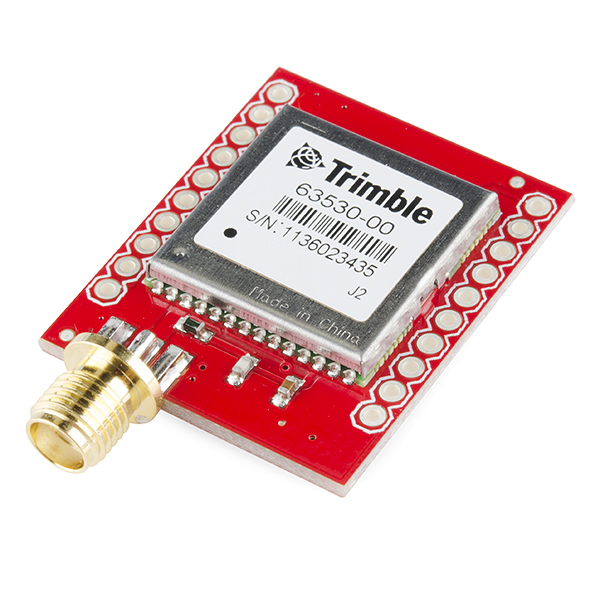
\includegraphics[width = 0.25\linewidth]{GPS_Copernicus}
\caption{\textit{Copernicus II GPS receiver}}
\label{fig:GPS_Copernicus}
\end{figure}

%\begin{landscape}
\begin{figure}[H]
\centering
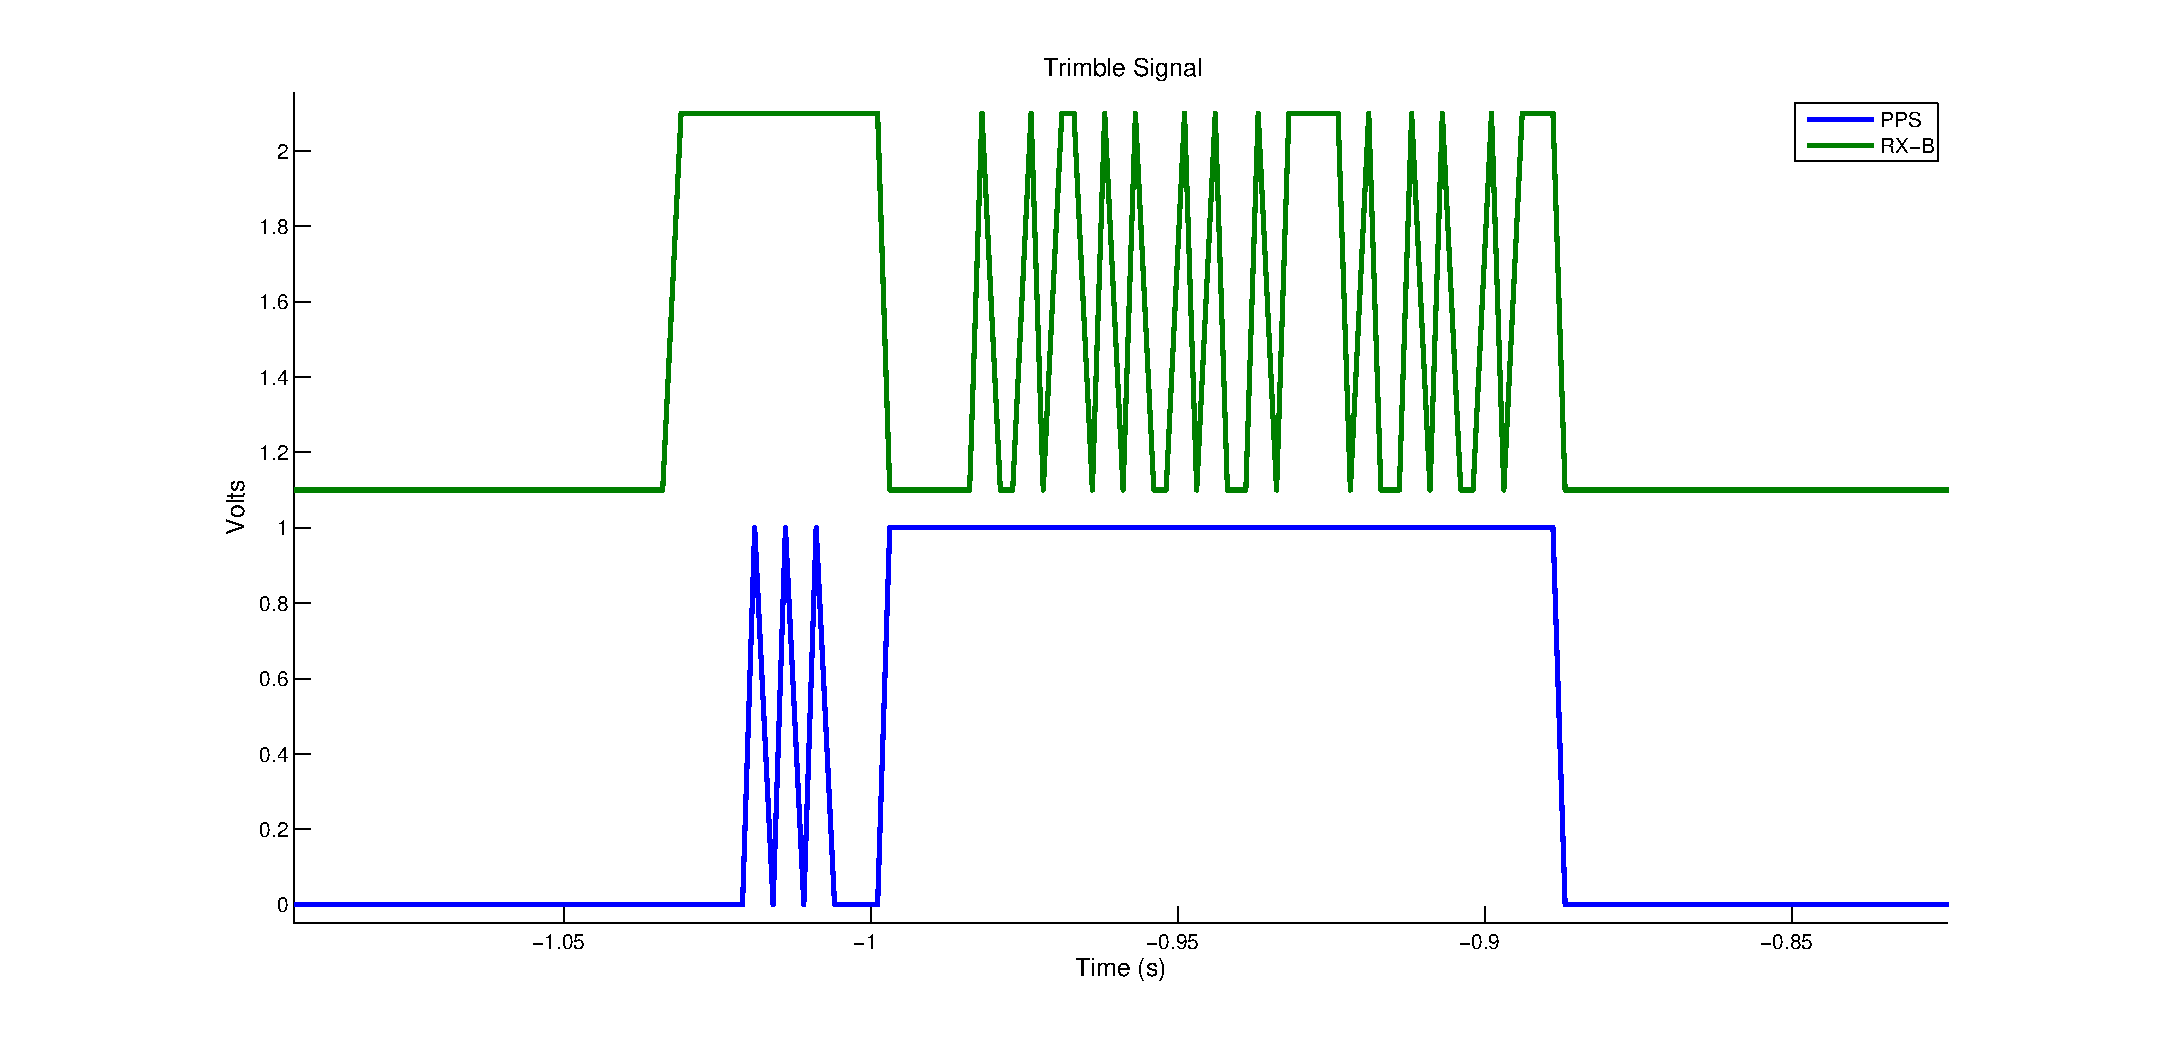
\includegraphics[width = 0.75\linewidth]{Trimble}
\caption{\textit{GPS sentence data and PPS signal recorded with oscilloscope for preliminary analysis.}}
\label{fig:GPS_PPS}
\end{figure}
%\end{landscape}